\documentclass[paper=a4, fontsize=11pt]{scrartcl} 

\usepackage[T1]{fontenc} 
\usepackage[english]{babel}
\usepackage{amsmath,amsfonts,amsthm}

\usepackage{lipsum}

\usepackage{graphicx}
\usepackage{float}
  \floatplacement{figure}{H}
  \floatplacement{table}{H}
  
\usepackage{sectsty} 
\allsectionsfont{\centering \normalfont\scshape} 

\usepackage{fancyhdr} % Custom headers and footers
\pagestyle{fancyplain} % Makes all pages in the document conform to the custom headers and footers
\fancyhead{} % No page header - if you want one, create it in the same way as the footers below
\fancyfoot[L]{} % Empty left footer
\fancyfoot[C]{} % Empty center footer
\fancyfoot[R]{\thepage} % Page numbering for right footer
\renewcommand{\headrulewidth}{0pt} % Remove header underlines
\renewcommand{\footrulewidth}{0pt} % Remove footer underlines
\setlength{\headheight}{13.6pt} % Customize the height of the header

\usepackage[labelformat=empty]{caption}
\usepackage{color}
\usepackage{listings}
\lstset{ %
language=bash,                % choose the language of the code
basicstyle=\footnotesize,       % the size of the fonts that are used for the code
numbers=left,                   % where to put the line-numbers
numberstyle=\footnotesize,      % the size of the fonts that are used for the line-numbers
stepnumber=1,                   % the step between two line-numbers. If it is 1 each line will be numbered
numbersep=5pt,                  % how far the line-numbers are from the code
backgroundcolor=\color{white},  % choose the background color. You must add \usepackage{color}
showspaces=false,               % show spaces adding particular underscores
showstringspaces=false,         % underline spaces within strings
showtabs=false,                 % show tabs within strings adding particular underscores
frame=single,           % adds a frame around the code
tabsize=2,          % sets default tabsize to 2 spaces
captionpos=b,           % sets the caption-position to bottom
breaklines=true,        % sets automatic line breaking
breakatwhitespace=false,    % sets if automatic breaks should only happen at whitespace
escapeinside={\%*}{*)}          % if you want to add a comment within your code
}



\numberwithin{equation}{section} % Number equations within sections (i.e. 1.1, 1.2, 2.1, 2.2 instead of 1, 2, 3, 4)
\numberwithin{figure}{section} % Number figures within sections (i.e. 1.1, 1.2, 2.1, 2.2 instead of 1, 2, 3, 4)
\numberwithin{table}{section} % Number tables within sections (i.e. 1.1, 1.2, 2.1, 2.2 instead of 1, 2, 3, 4)

\setlength\parindent{0pt} % Removes all indentation from paragraphs - comment this line for an assignment with lots of text

%----------------------------------------------------------------------------------------
%	TITLE SECTION
%----------------------------------------------------------------------------------------

\newcommand{\horrule}[1]{\rule{\linewidth}{#1}} % Create horizontal rule command with 1 argument of height

\title{	
\normalfont \normalsize 
\textsc{Computational Science - ITB} \\ [25pt] % Your university, school and/or department name(s)
\horrule{0.5pt} \\[0.4cm] % Thin top horizontal rule
Random Walk Foton di Zona Radiasi Matahari\\ % The assignment title
%\horrule{2pt} \\[0.5cm] % Thick bottom horizontal rule
}

\author{\small{Febrie Ahmad Azizi || 20912008} \\ \small{Ridlo W. Wibowo || 20912009}} % Your name
\date{\normalsize December 15, 2012} % Today's date or a custom date

\begin{document}

\maketitle % Print the title

\large \textbf{Dokumentasi.}\\
Program untuk menyimulasikan pergerakan random walk foton di Zona Radiasi Matahari kami buat dengan sederhana. Algoritmanya dapat dijelaskan sebagai berikut:
\begin{enumerate}
\item Inisiasi, $r = 0$ atau $(0,0,0)$, dan $t = 0$ 
\item Acak \textit{uniform} arah dalam koordinat Bola.
\item Acak tempat terjadi \textit{collision} ($r_{col}$) dengan mengunakan aturan yang akan dijelaskan dibawah (\textit{tracking}).
\item Update waktu foton berjalan ($t$).
\item Tentukan posisi baru foton dengan transformasi koordinat kartesian menggunakan $r_{col}$ dan arah geraknya.
\item Hitung dan update $r$ baru.
\item Bandingkan $r$ dengan $R_{rad}$, jika $r \geq R_{rad}$ STOP.
\item Ulangi ke langkah no 2. 
\item Hitung perbandingan waktu cahaya berjalan secara $randomwalk$ dengan foton berjalan lurus sejauh $R_{rad}$, kita sebut sebagai $t_{mode,scale} = \frac{t}{R_{rad}/c}$, $ c = $ kecepatan cahaya.
\end{enumerate}

\newpage
\textbf{	\textit{Source}}\\
Untuk membuat random arah yang \textit{uniform} saat awal simulasi ($r = 0$) dan arah baru setelah terjadi tumbukan, maka dibuat random dalam koordinat bola. Posisi atau vektor dalam ruang 3D dapat dinyatakan dengan koordinat Bola ($r, \phi, \theta$), dengan transformasi ke koordinat kartesian dapat menggunakan:
\begin{equation*}
x = r \sin\theta \cos\phi
\end{equation*}
\begin{equation*}
y = r \sin\theta \sin\phi
\end{equation*}
\begin{equation*}
z = r \cos\theta
\end{equation*}

Luas sudut permukaan Bola adalah $\Omega = 4\pi$ steradian.
\begin{equation*}
F(\Omega) = \int_{0}^{\Omega} \frac{d\Omega}{4\pi}
\end{equation*}
\begin{equation*}
F(\theta, \phi) = \frac{1}{4\pi} \int_{0}^{\theta} \int_{0}^{\phi} \sin \theta d\theta d\phi
\end{equation*}
\begin{equation*}
F(\theta, \phi) = \frac{1}{4\pi} \int_{0}^{\theta} \sin \theta d\theta \int_{0}^{\phi} d\phi
\end{equation*}
\begin{equation*}
F(\theta, \phi) = \frac{1}{4\pi} (1 - \cos \theta) \phi
\end{equation*}
sehingga diperoleh,
\begin{equation*}
F(\theta) = \frac{1}{2} (1 - \cos \theta) = r_{1}
\end{equation*}
\begin{equation*}
F(\phi) = \frac{\phi}{2\pi} = r_{2}
\end{equation*}
atau,
\begin{equation*}
\theta = \arccos (1 - 2 r_{1})
\end{equation*}
\begin{equation*}
\phi = 2 \pi r_{2}
\end{equation*}

Perbandingan random dengan aturan di atas dan dengan mengambil random langsung untuk sudutnya ($ 0 < r_1 < \pi,  0 < r_2 < 2\pi$) yang akan mengakibatkan lebih banyak titik/arah pada kutubnya ditunjukkan pada gambar di bawah ini,
\begin{figure}
	\centering
	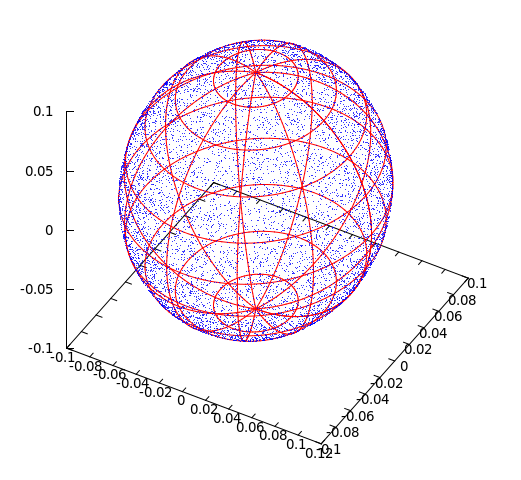
\includegraphics[width=0.48\textwidth]{distribusibola-benar.png}
	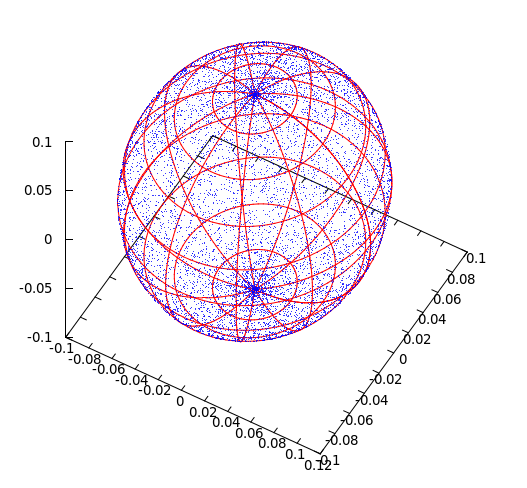
\includegraphics[width=0.48\textwidth]{distribusibola-salah.png}
	\caption{(kiri) distribusi \textit{uniform} yang benar, (kanan) distribusi tidak \textit{uniform}.}
\end{figure}


\vspace{1.5cm}
\textbf{\textit{Tracking}}\\
Bagian ini berguna untuk menentukan seberapa jauh foton bergerak sebelum menumbuk elektron, sehingga faktor utama yang mempengaruhi adalah \textit{mean free path} dari foton saat berada di zona radiasi Matahari. Telah dijelaskan di laporan, pendekatan dilakukan untuk menyimulasikan kasus ini, karena yang kita ingin tentukan hanya waktu yang dibutuhkan foton untuk keluar dari zona radiasi. Penyederhanaan itu dilakukan dengan menggunakan teori klasik yaitu \textit{Thomson scattering} untuk menentukan \textit{mean free path} foton. Telah diketahui pula bahwa \textit{cross-section} foton terhadap elektron jauh lebih besar dibandingkan dengan proton.

\textit{Mean free path} ($f$) foton ditentukan dengan:
\begin{equation*}
f = \frac{m_e + m_p}{\sqrt{2} \sigma_T \rho}
\end{equation*}
dengan $\sigma_T$ merupakan \textit{Thomson cross-section} sebesar $6.65245854533 \times 10^{-29}$ m$^2$, dan $\rho$ merupakan kerapatan zona radiasi ($\rho_r$ untuk kasus model kerapatan linear).\\

Kemudian kita harus menentukan sejauh apa foton dapat bergerak lurus setelah tumbukan ($r_{col}$), tentunya kita dapat buat random jarak yang apabila kita rata-ratakan untuk banyak percobaan harus mendekati kembali nilai $f$ yang sudah ditentukan di atas.\\

\textit{Penurunan mean free path}\\
Dapat kita bayangkan apabila terdapat sinar atau partikel yang bergerak melintasi kumpulan partikel lain, maka penampang melintang permukaan ($slab$) yang ia lewati dapat digambarkan seperti dibawah ini.
\begin{figure}
	\centering
	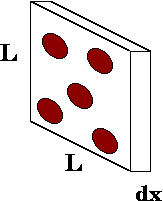
\includegraphics[width=0.2\textwidth]{mfp.png}
\end{figure}
Luas permukaan $slab$ adalah $L^2$ dan volumenya $L^2 dx$, sedangkan luas penampang partikel total adalah $\sigma n L^2 dx$ dengan $n$ adalah jumlah partikel per satuan volum. Probabilitas tumbukan dengan sistem partikel untuk selang $dx$ menjadi,
\begin{equation*}
P(berhenti setelah dx) = \frac{area partikel}{area slab} = \frac{\sigma n L^2 dx}{L^2} = \sigma n dx
\end{equation*}

Perubahan intensitas sinar atau jumlah partikel yang menerobos adalah
\begin{equation*}
dI = -I \sigma n dx
\end{equation*}
atau,
\begin{equation*}
\frac{dI}{dx} = -I \sigma n \equiv^{def} -\frac{I}{f}
\end{equation*}
didefinisikan bahwa $f$ adalah \textit{mena free path} yaitu jarak rata-rata perjalanan sebelum partikel menumbuk partikel lain.

Dari persamaan di atas diperoleh solusi $I = I_0 e^{-x/f}$ sehingga perubahan probabilitas tumbukan untuk selang $dx$ adalah
\begin{equation*}
dP(x) = \frac{I(x) - I(x+dx)}{I_0} = \frac{1}{f} e^{-x/f} dx
\end{equation*}
dan nilai ekspektasi (atau rata-rata) dari x menjadi
\begin{equation*}
<x> =^{def} \int_0^{\infty} x dP(x) = \int_0^{\infty} \frac{x}{f} e^{-x/f} dx = f
\end{equation*}

Oleh karena itu untuk mendapatkan random yang sesuai dapat diperoleh dari,
\begin{equation*}
F(x) = \int_0^x \frac{1}{f} e^{-x/f} dx = 1 - e^{-x/f}
\end{equation*}
dengan demikian jarak tumbukan ($r_{col}$) dapat ditentukan,
\begin{equation*}
r_{col} = x = -f \ln (1-r_3)
\end{equation*}
atau, karena $r_3$ merupakan random \textit{uniform} antara 0 dan 1, maka dapat pula kita ganti menjadi
\begin{equation*}
r_{col} = -f \ln r_3
\end{equation*}

\vspace{1.5cm}
\textbf{\textit{Program}}\\
Program dibuat dan dijalankan untuk \textit{single-processor} dan \textit{multi-processor} (menggunakan \textit{OpenMPI}). Kami membagi pekerjaan yang sama untuk dijalankan di masing-masing \textit{processor} dengan hanya membedakan \textit{seed} bilangan randomnya (pseudo. Untuk parameter yang sama kami perlu menjalankan $1000$ kali dengan \textit{seed} random yang berbeda, sehingga kami cukup membagi rata sesuai jumlah \textit{processor} (dalam hal ini jumlah $thread$ yang tersedia). Program terlampir di bawah, sedangkan hasil simulasi dan tabel waktu komputasi diberikan di laporan.

\textit{Screenshot} $htop$ (ubuntu) untuk melihat kinerja $processor$ untuk program yang sama.
\begin{figure}
	\centering
	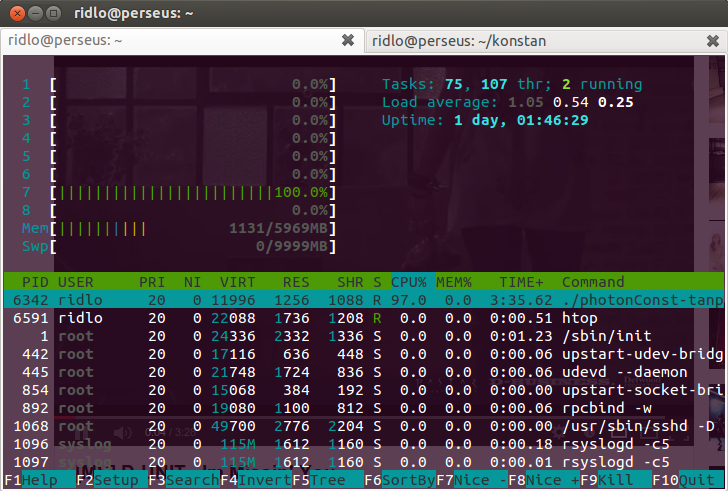
\includegraphics[width=0.7\textwidth]{htop-konstan-tanpaMPI.png}\\
	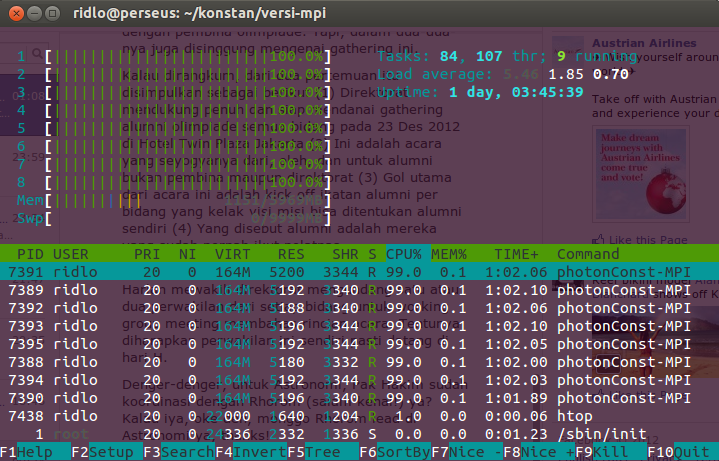
\includegraphics[width=0.7\textwidth]{htop-konstan-MPI.png}
	\caption{$htop$, (atas) tanpa MPI, dan (bawah) dengan MPI untuk 4 \textit{core} \--- 8 \textit{threads}.}
\end{figure}


\vspace{1.5cm}
\textbf{Lampiran Program}\\
\textbf{Model kerapatan konstan \--- tanpa MPI}\\
\lstset{frameround=fttt}
\begin{lstlisting}
#include <iostream>
#include <stdio.h>
#include <math.h>
#include <fstream>
#include <stdlib.h>
#include <time.h>
#include <ctime>
#include <string>
#define _USE_MATH_DEFINES
#define c 299792458.
using namespace std;

double unirand(){return (double) rand()/(double) RAND_MAX;}

double randomwalk(double Rrad){
    double r, theta, phi, x, y, z, dx, dy, dz, f, rho, dt, t, rcol, randcol;
    double me = 9.11e-31; // kg
    double mp = 1.67e-27; // kg
    double sigmaT = 6.65245854533e-29; // m^2
    unsigned int n=0;
    x = 0.0; y = 0.0; z = 0.0, t=0.0, dt=0.0; 
    rho = 15000.; // Constant Density
    f = (me+mp)/(sqrt(2.)*sigmaT*rho);
    do{ 
            phi = 2.*M_PI*unirand(); theta = acos(1.-2.*unirand());
            do{
                randcol = unirand();
            } while (randcol == 0.0 || randcol == 1.0); // menghindari -inf
            rcol = -f*log(randcol);
            dt = rcol/c;
            t = t+dt;
            dx = rcol*sin(theta)*cos(phi); 
            dy = rcol*sin(theta)*sin(phi); 
            dz = rcol*cos(theta);
            x=x+dx; 
            y=y+dy; 
            z=z+dz;
            n = n+1;
            r = sqrt(x*x + y*y + z*z);
    } while (r <= Rrad);
    
    double tm = t/(Rrad/c);
    return tm;
}

int main(int argc, char** argv){
    time_t tstart=time(0), tend, tim, start, finish;
    clock_t begin, end;
    int N = 1000;
    double R[7]={0.05,0.1,0.2,0.5,1.0,2.0,5.0};
    
    for (int j=0;j<7;j++){
        // inisiasi timer
        if (R[j] < 1.0){ begin = clock();}
        else { start = time(0);}
        
        // progran utama
        char filename[64];
        double Rrad=R[j];
        srand(time(NULL));
        sprintf(filename, "out-photonConst%d.txt", j);
        ofstream out(filename);
        for (int i=0;i<N;i++){
            out << randomwalk(Rrad) << endl;
        }
        
        // end timer
        if (R[j] < 1.0){
            end = clock();
            out << "running time = " << (double)(end - begin)/(double)CLOCKS_PER_SEC << " seconds." << endl;
        }
        else { 
            finish = time(0);
            out << "running time = " << (double)(finish - start) << " seconds." << endl;
        }
        out.close();
    }
    tend = time(0);
    tim = tend - tstart;
    cout << "running time = " << tim/60. << " minutes." << endl;
    return 0;
}
\end{lstlisting}

\vspace{1.5cm}
\textbf{Model kerapatan konstan \--- dengan MPI}\\
\lstset{frameround=fttt}
\begin{lstlisting}
#include <iostream>
#include <stdio.h>
#include <math.h>
#include <fstream>
#include <stdlib.h>
#include <time.h>
#include <ctime>
#include <string>
#include <mpi.h>
#define _USE_MATH_DEFINES
#define c 299792458.
using namespace std;

double unirand(){return (double) rand()/(double) RAND_MAX;}

double randomwalk(double Rrad){
    double r, theta, phi, x, y, z, dx, dy, dz, f, rho, dt, t, rcol, randcol;
    double me = 9.11e-31; // kg
    double mp = 1.67e-27; // kg
    double sigmaT = 6.65245854533e-29; // m^2
    unsigned int n=0;
    x = 0.0; y = 0.0; z = 0.0, t=0.0, dt=0.0; 
    rho = 15000.; // Constant Density
    f = (me+mp)/(sqrt(2.)*sigmaT*rho);
    do{ 
            phi = 2.*M_PI*unirand(); theta = acos(1.-2.*unirand());
            do {
                randcol = unirand();
            } while (randcol == 0.0 || randcol == 1.0); // mengindari -inf
            rcol = -f*log(randcol);
            dt = rcol/c;
            t = t+dt;
            dx = rcol*sin(theta)*cos(phi); 
            dy = rcol*sin(theta)*sin(phi); 
            dz = rcol*cos(theta);
            x=x+dx; 
            y=y+dy; 
            z=z+dz;
            n = n+1;
            r = sqrt(x*x + y*y + z*z);
    } while (r <= Rrad);
    
    double tm = t/(Rrad/c);
    return tm;
}

int main(int argc, char** argv){
    time_t tstart=time(0), tend, tim;
    int m = 8;
    int N = 125;
    double R[7]={0.05, 0.1, 0.2, 0.5, 1.0, 2.0, 5.0};

        int rank, nprocs;
        MPI_Init(&argc, &argv);
        MPI_Comm_size(MPI_COMM_WORLD, &nprocs);
        MPI_Comm_rank(MPI_COMM_WORLD, &rank);
    
    for (int k=0;k<7;k++){
        double Rrad=R[k];
        for (int j=0;j<m;j++){
            if (rank == j){
                clock_t begin, end;
                time_t start, finish;
                if (Rrad < 1.0){ begin = clock();}
                else { start = time(0);}
                char filename[64];
                srand(time(NULL)+7+j);
	        sprintf(filename, "outfile-MPI-%d-%d.txt", k, j);
                ofstream out(filename);
                for (int i=0;i<N;i++){
                    out << randomwalk(Rrad) << endl;
                }
                if (R[k] < 1.0){ 
                    end = clock();
                    out << "running time = " << (double)(end - begin)/(double)CLOCKS_PER_SEC << " seconds." << endl;
                }
                else {
                    finish = time(0);
                    out << "running time = " << (double)(finish - start) << " seconds." << endl;
                }
                out.close();
            }
        }
    }
        MPI_Finalize();
    tend = time(0);
    tim = tend - tstart;
    cout << "running time = " << tim/60. << " minutes." << endl;
    return 0;
}
\end{lstlisting}


\vspace{1.5cm}
\textbf{Model kerapatan linear \--- dengan MPI}\\
\lstset{frameround=fttt}
\begin{lstlisting}
#include <iostream>
#include <stdio.h>
#include <math.h>
#include <fstream>
#include <stdlib.h>
#include <time.h>
#include <ctime>
#include <string>
#include <mpi.h>
#define _USE_MATH_DEFINES
#define c 299792458.
using namespace std;

double unirand(){return (double) rand()/(double) RAND_MAX;}

double randomwalk(double Rrad){
    double r, theta, phi, x, y, z, dx, dy, dz, f, rho, dt, t, rcol, randcol;
    double me = 9.11e-31; // kg
    double mp = 1.67e-27; // kg
    double sigmaT = 6.65245854533e-29; // m^2
    unsigned int n=0;
    x = 0.0; y = 0.0; z = 0.0, t=0.0, dt=0.0, r=0.0; 
    do{ 
            rho = -3e4*5.*r/Rrad + 1.5e5; // linier gradient density
            f = (me+mp)/(sqrt(2.)*sigmaT*rho);
            phi = 2.*M_PI*unirand(); theta = acos(1.-2.*unirand());
            do {
                randcol = unirand();
            } while (randcol == 0.0 || randcol == 1.0); // menghindari -inf
            rcol = -f*log(randcol);
            dt = rcol/c;
            t = t+dt;
            dx = rcol*sin(theta)*cos(phi); 
            dy = rcol*sin(theta)*sin(phi); 
            dz = rcol*cos(theta);
            x=x+dx; 
            y=y+dy; 
            z=z+dz;
            n = n+1;
            r = sqrt(x*x + y*y + z*z);
    } while (r <= Rrad);
    
    double tm = t/(Rrad/c);
    return tm;
}

int main(int argc, char** argv){
    time_t tstart=time(0), tend, tim;
    int m = 8;
    int N = 125;
    double R[7]={0.05, 0.1, 0.2, 0.5, 1.0, 2.0, 5.0};

        int rank, nprocs;
        MPI_Init(&argc, &argv);
        MPI_Comm_size(MPI_COMM_WORLD, &nprocs);
        MPI_Comm_rank(MPI_COMM_WORLD, &rank);
    
    for (int k=0;k<7;k++){
        double Rrad=R[k];
        for (int j=0;j<m;j++){
            if (rank == j){
                clock_t begin, end;
                time_t start, finish;
                if (Rrad < 1.0){ begin = clock();}
                else { start = time(0);}
                char filename[64];
                srand(time(NULL)+7+j);
	        sprintf(filename, "outfile-lin-MPI-%d-%d.txt", k, j);
                ofstream out(filename);
                for (int i=0;i<N;i++){
                    out << randomwalk(Rrad) << endl;
                }
                if (R[k] < 1.0){ 
                    end = clock();
                    out << "running time = " << (double)(end - begin)/(double)CLOCKS_PER_SEC << " seconds." << endl;
                }
                else {
                    finish = time(0);
                    out << "running time = " << (double)(finish - start) << " seconds." << endl;
                }
                out.close();
            }
        }
    }
        MPI_Finalize();
    tend = time(0);
    tim = tend - tstart;
    cout << "running time = " << tim/60. << " minutes." << endl;
    return 0;
}
\end{lstlisting}
\end{document}